\subsection{Miscellaneous}

\begin{frame}{OpenMPI}
\begin{columns}
    \begin{column}{.5 \textwidth}

    \textbf{\large Modular Component Architecture(MCA)}

    \begin{itemize}
        \item MCA framework
        \item MCA component
        \item MCA module
    \end{itemize}
            
    \end{column}

    \begin{column}{.5 \textwidth}
        \begin{figure}
            \centering
            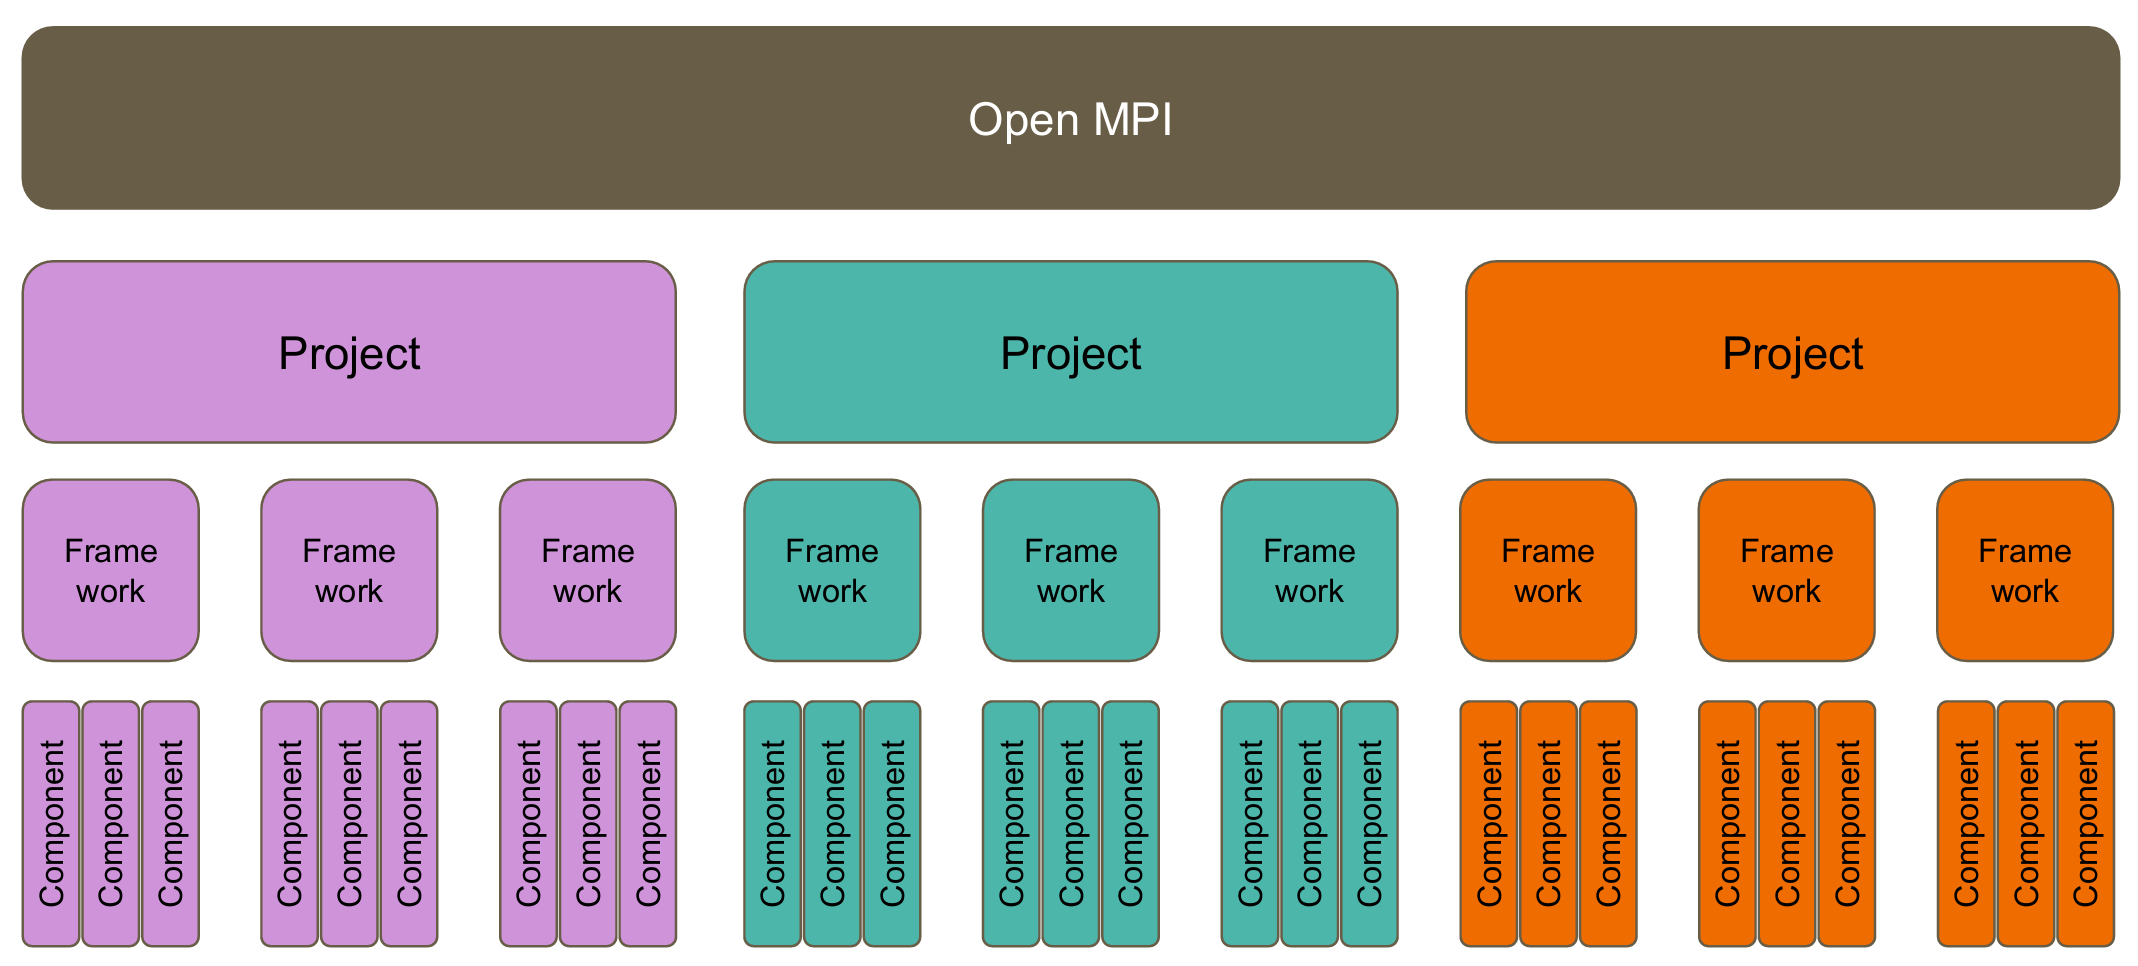
\includegraphics[width=1\linewidth]{day8_am/img/mpi/ompi_arch.png}
            \caption{OpenMPI Overall Architecture Terminology}
            \label{fig:ompi_arch}
        \end{figure}
    \end{column}    
\end{columns}
\end{frame}

\begin{frame}{OpenMPI}
\begin{columns}
    \begin{column}{.5 \textwidth}

    \textbf{\small 3 Types of OpenMPI Framework}

    \begin{itemize}
        \item In the MPI layer (OMPI)
        \item In the run-time layer (ORTE)
        \item In the operating system/platform layer (OPAL)
    \end{itemize}


    You might think of these frameworks as ways to group MCA parameters by function. (e.g. btl in OMPI)

    
    \end{column}

    \begin{column}{.5 \textwidth}
        \begin{figure}
            \centering
            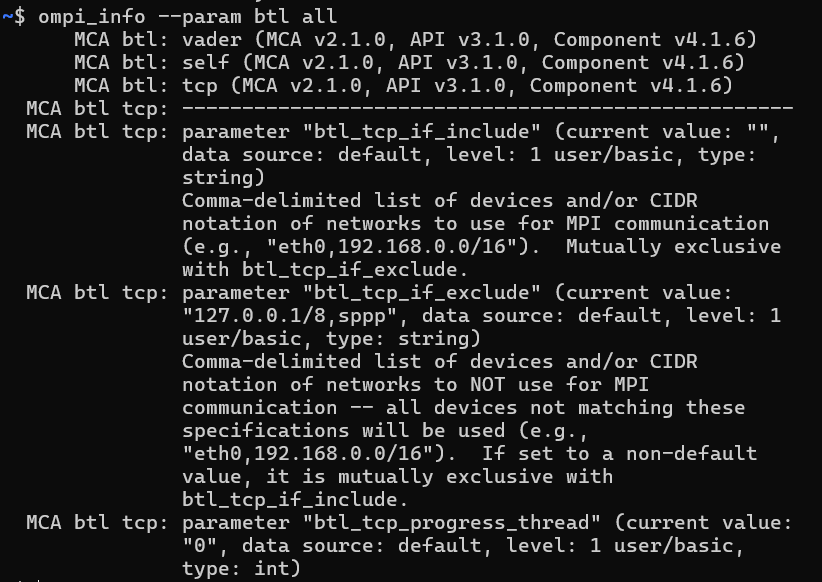
\includegraphics[width=1\linewidth]{day8_am/img/mpi/ompi_info.png}
            \caption{ompi\_info}
            \label{fig:ompi_info}
        \end{figure}
    \end{column}    
\end{columns}
\end{frame}

\begin{frame}[fragile]{OpenMPI(Installation) cont.}
\begin{columns}
    \begin{column}{.5 \textwidth}

    \textbf{\small Specify Compilers}
    
    {\scriptsize ./configure CC=/path/to/clang \\}

    {\scriptsize CXX=/path/to/clang++ FC=/path/to/gfortran ...}

    \vspace{1cm}
      \textbf{\small Static or Shared ?}
    {\scriptsize \begin{itemize}
        \item --enable-static / --disable-static (default)

        libmpi.a

        \item --enable-shared / --disable-shared

        libmpi.so
    \end{itemize}}
    \end{column}

    
    
    \begin{column}{.5 \textwidth}
        \textbf{\small Communication Library}
        
        UCX (Unified Communication X)

        {\scriptsize --with-ucx[=UCX\_INSTALL\_DIR]}
        
        \vspace{1cm}
        
        \textbf{\small With CUDA support}

        {\scriptsize ./configure --with-cuda[=/path/to/cuda]}
    \end{column}    
\end{columns}
\end{frame}

\begin{frame}[fragile]{OpenMPI (mpirun)}

\begin{itemize}
    \item -x [env]

    Passes environment variables to remote nodes.

    \item --bind-to core

    \item -hostfile [hostfile]

    \item ...
\end{itemize}
\end{frame}

% \begin{frame}{Loading MPI On Our Cluster}
% \begin{itemize}
%     \item \$ module load openmpi/5.0.3-pe46zvn
%     \item \$ module load intel-oneapi-mpi/2021.13.0-hpxfbao
% \end{itemize}
% \end{frame}

% \begin{frame}{Profiling and Tuning MPI Programs}
%     Later lectures. (7.12)
% \end{frame}